\documentclass[12pt, a4paper]{article}
\usepackage{../notesheets}

%%%%%%%%%%%%%%%%%%%%%%%%%%%%%%%%%%%%%%%%%%%%%%%%%%
\author{Math 1210}
\title{Notesheet. Section 3.6: Implicit Differentiation}
\date{}

\begin{document}
\maketitle
\nameline
%%%%%%%%%%%%%%%%%%%%%%%%%%%%%%%%%%%%%%%%%%%%%%%%%%
\begin{defi}
  An \de{explicit} relationship between independent variable \(x\) and
  a dependent variable \(y\) is a relationship of the form \(y = f(x)\), such as \(y
  = \sqrt{x^3+1}\) or \(y = 5x^2+7x+1\). An \de{implicit} relationship
  between an independent variable \(x\) and dependent variable \(y\) is
\end{defi}
\begin{ex}
  What is an equation whose solution is a circle of radius \(2\)
  centered at the origin, \((0,0)\). Is this equation an implicit or
  explicit relationship between \(x\) and \(y\)?
\end{ex}
\begin{ex}
  If \(x^2 + y^2 = 25\), what is \(\frac{dy}{dx}\)? What is an
  equation of the tangent line to the circle \(x^2+y^2=25\) at the
  point \((3,4)\)? Hint: Do not solve for \(y\) in terms of
  \(x\). Instead, assume \(y\)
  is a function of \(x\), say \(y = f(x)\), and use the chain
  rule. Your final answer may be in terms of \(x\) and \(y\).
\end{ex}
\vspace{-0.5in}
\begin{defi}
  The process of finding the derivative \(\frac{dy}{dx}\) from an
  implicit relationship between \(x\) and \(y\) is called \de{implicit
    differentiation}.
\end{defi}
\begin{ex}
  Let \(x^3 + y^3 = 6xy\) be the ``folium of Descartes''. What is \(y'\)? Find the tangent line to
  the folium at the
  point \((3,3)\). At what points in the first quadrant is the tangent
  line horizontal?
\end{ex}
\begin{ex}
  In the ``Lots of Derivatives'' notesheet, you were asked the
  following question. Air is being pumped into a spherical weather
  balloon. At any time
  \(t\), the volume of the balloon is \(V(t)\) and its radius is
  \(r(t)\). Recall that, for a sphere, \(V = \frac{4}{3} \pi
  r^3\). What is \(\frac{dV}{dt}\) in terms of \(r(t)\) and
  \(r'(t)\)?
\end{ex}
\begin{defi}
  In the above problem, finding \(\frac{dV}{dt}\) required using \(r'(t)\) in
  your final answer. This is a related rate. A \de{related rate} is
\end{defi}
\begin{ex}
  A water tank has the shape of an inverted circular cone with base
  radius \(2\)m and height \(4\)m. If water is being pumped into the
  tank at a rate of \(2\) cubic meters/minute, find the rate at which
  the water level is rising when the water is \(3\)m deep.
\end{ex}
\vspace{-2.2in}
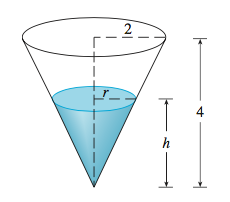
\includegraphics[scale=0.5]{images/conic-water-tank}
%%%%%%%%%%%%%%%%%%%%%%%%%%%%%%%%%%%%%%%%%%%%%%%%%%
\end{document}
